% !TEX root = ../main.tex
\subsection{Cuts} \label{ssec::cuts}
    Three types of cuts are applied to particles to increase their value for the analysis provided in this work:
    \begin{itemize}
        \item
            General cuts, which exclude badly reconstructed particles.
        \item
            Geometry cuts, which limit the region from where reconstruction data is useful for this analysis.
        \item
            DIS cuts, which limit the region of analysis to that of DIS.
    \end{itemize}

% --+ General cuts +------------------------------------------------------------
    Only two cuts are considered ``general'' for this analysis.
    The first one simply filters out particles with PID $0$ or $45$.
    These PIDs are used in CLAS12 reconstruction to denote particles whose PID couldn't be successfully identified.
    Then, the second filters out particles whose tracking is not very precise, and is defined as
    \begin{equation*}
        \frac{\chi^2}{\text{NDF}} < 15,
    \end{equation*}
    where $\chi^2$ is the final result from the $\chi^2$-test used to guide the Kalman filter fit in the tracking algorithm, as described in \ref{sssec::offlinereconstruction}, and NDF is the number of degrees of freedom of this same fit.

    \begin{figure}[b!]
        \centering\frame{
        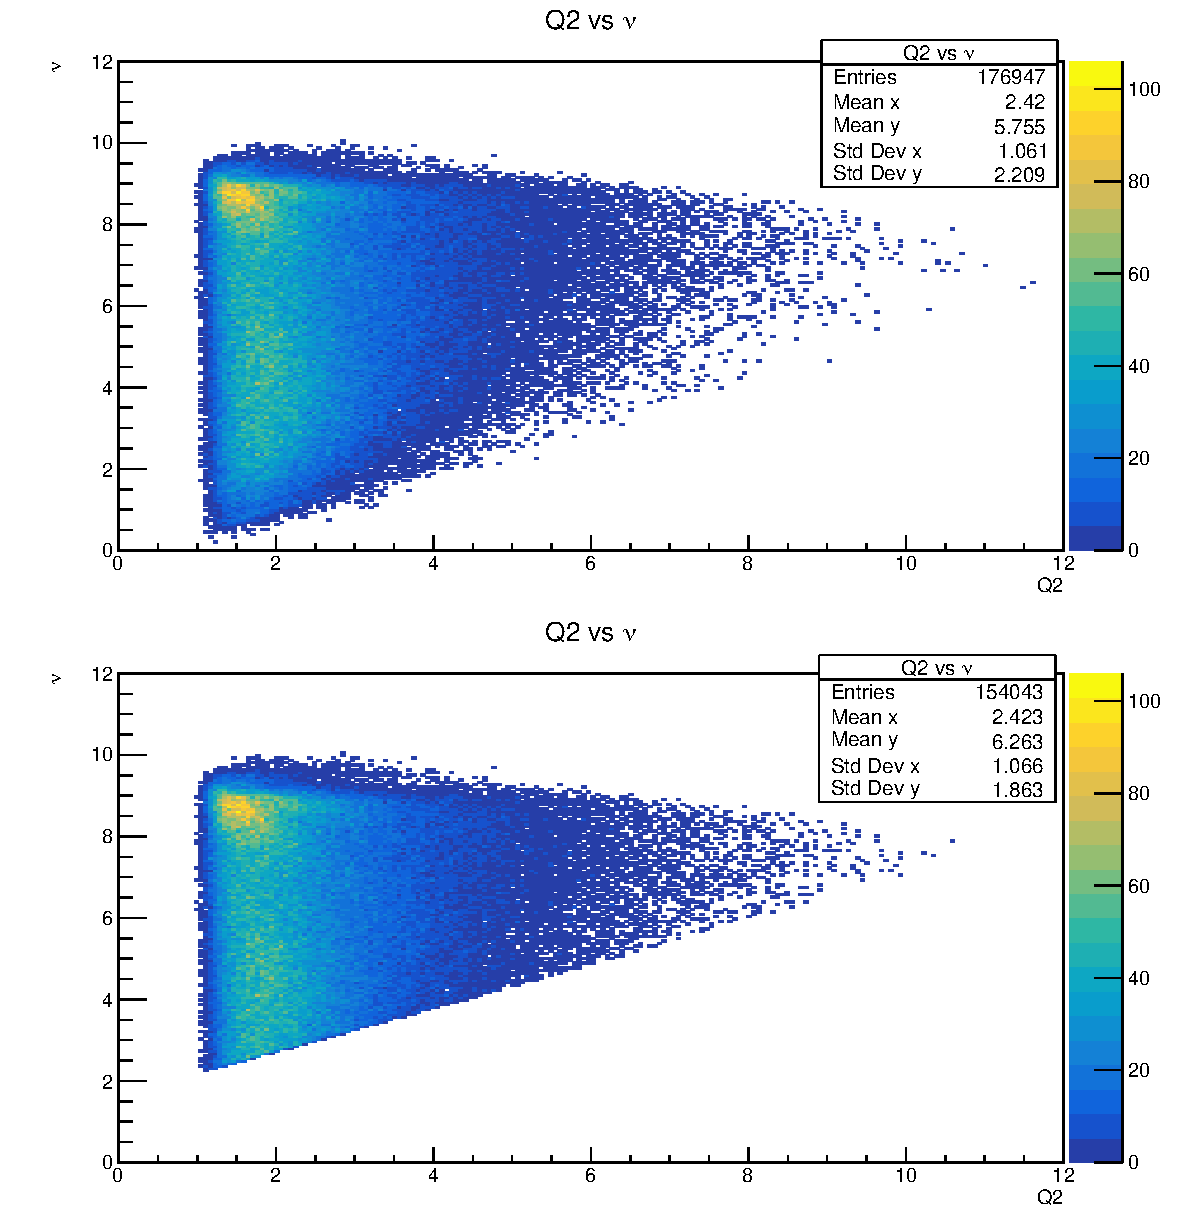
\includegraphics[width=\textwidth]{13dataanalysis/img/20q2_vs_nu.pdf}}
        \caption[$Q^2$ vs $\nu$ comparison]{$Q^2$ vs $\nu$ before and after applying the $Q^2 > 1$ and $W^2 > 4$ cuts.}
        \label{fig::q2vsnu}
    \end{figure}

% --+ Geometry cuts +-----------------------------------------------------------
    The geometry cuts also include two cuts, both working to constrain the vertex of the reconstructed particle to the beamline.
    The first one secures us that the vertex comes from the beamline, and is given by
    \begin{equation*}
        \sqrt{v_x^2 + v_y^2} < 4 \text{ cm},
    \end{equation*}
    where $v_x$ and $v_y$ are the $x$ and $y$ coordinates of the vertex position.
    The second one ensures that the hit comes from the target, and is
    \begin{equation*}
        -40 \text{ cm} < v_z < 40 \text{ cm},
    \end{equation*}
    where $v_z$ is the $z$ coordinate of the vertex position.
    This cut is defined from the shape of the RG-F target.

% --+ DIS cuts +----------------------------------------------------------------
    Finally, the DIS cuts are cuts made on the scattered electron to limit the phase space to that of DIS.
    All particles in an event are ignored if the trigger electron doesn't pass these cuts.

    First, a cut is applied on the invariant mass of the virtual photon, $Q^2$, which is
    \begin{equation*}
        Q^2 > 1 \text{ GeV}^2,
    \end{equation*}
    ensuring that we are in the domain of DIS.

    Then, a cut is made on the squared mass of the hadronic final state, $W^2$, given by
    \begin{equation*}
        W^2 > 4,
    \end{equation*}
    where $W^2$ is defined by
    \begin{equation*}
        W^2 = M^2 + 2M\nu - Q^2,
    \end{equation*}
    and $M$ is the nucleon mass, and $\nu$ is the energy fraction of the virtual photon.
    This cut is applied to exclude nucleon resonances.

    The effect of these cuts on $Q^2$ and $\nu$ can be seen on plot \ref{fig::q2vsnu}.
